% !TEX root = dissertation_BB.tex
%% spellcheck-language en-US

%  ####
%      #
%   ###
%  #
%  #####

\chapter{Dual Mouse-SPIM}

\graphicspath{{./figures/2_DualMouse/}}

\section{Previous Mouse-SPIM}
mammalian development
chromosome segregation
cell specification
symmetry breaking
signaling pathways
human infertility
congenital diseases 

current mouse-SPIM \cite{strnad_inverted_2016} already is very good for answering many of these questions

advantages:
    immersion liquid and culture medium separated
    open-top sample holder allow standard microdrop \textit{in vitro} embryo culture
    row of embryos - high throughput
    dual color imaging
    environmental chamber allows live imaging for 3 days, every 

follow chromosomes by tracking kinetochores

from lattice paper: ``because photodamage mechanisms that scale supralinearly with peak intensity have been identified for both visible \cite{donnert_major_2007} and two-photon \cite{ji_high-speed_2008} excitation."



\section{Light collection efficiency of an objective}
Resolution is not the only parameter of concern when designing a new microscope setup. We also have to consider light collection efficiency, since many application, especially live imaging applications require a tight photon budget. This means a single fluorophore can only emit so many times before it undergoes an irreversible chemical reaction, i.e. it bleaches. The more we can collect of these photons, the more information we gain, and altogether the efficiency is higher.

Photon collection efficiency also defines single molecule localization accuracy, since the signal to noise ratio will depend on the square of the number of collected photons. This is why it's important to also maximize light collection efficiency.

Let's define light collection efficiency $\eta$ as the ratio of collected photons and all emitted photons:
\[
\eta = \frac{N_{collected}}{N_{emitted}}
\]
Since we can assume that the direction of photons emitted from a fluorescent molecule are random, the light collection efficiency will correspond to the solid angle subtended by the objective front lens at the focal point. To calculate this, let's consider the unit sphere centered at the focal point, and calculate the surface area of the spherical cap corresponding to the objective acceptance angle $\alpha$ (Fig. \ref{fig:light_effa}). The area of the cap can be expressed as a function of the angle:
\[
A_{cap} = 2\pi r^2 (1-\cos \alpha)
\]
The surface area of the full sphere is calculated as:
\[
A_{sph} = 4 \pi r^2
\]
For both equations $r$ is the radius of the sphere. From here, the light collection efficiency can be calculated as:
\[
\eta = \frac{N_{collected}}{N_{emitted}} = \frac{A_{cap}}{A_{sph}} = \frac{1-\cos \alpha}{2}
\]

Some more calculations: (Fig. \ref{fig:light_effb}).

\begin{figure}[tpb]
\begin{subfigure}[t]{0.49\textwidth}
    \centering
    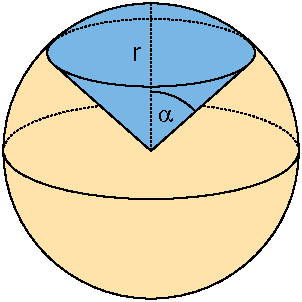
\includegraphics[page=1,width=0.8\textwidth]{efficiency/sphere}
    \caption{\textbf{}}
    \label{fig:light_effa}
\end{subfigure}
\begin{subfigure}[t]{0.49\textwidth}
    \centering
    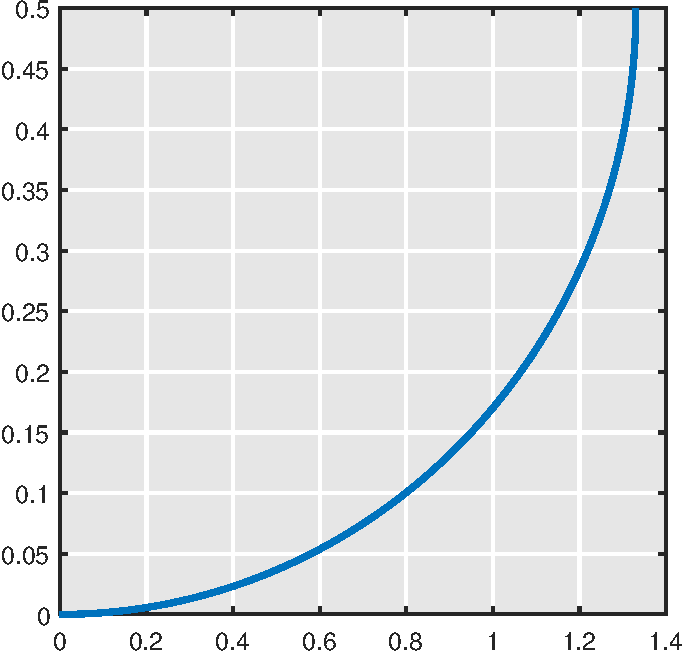
\includegraphics[page=1,width=1\textwidth]{efficiency/light_eff}
    \caption{\textbf{}}
    \label{fig:light_effb}
\end{subfigure} 
 \bcaption[Light collection efficiency of an objective]{\textbf{(a)} Light collection efficiency is the ratio of photons collected by the objective and all emitted photons. If the fluorophores are emitted randomly in all directions, it will be the surface ratio of the conical section (blue) to the whole sphere. \textbf{(b)} Light collection efficiency ($\eta$) as a function of the numerical aperture (NA)}
 \label{fig:light_eff}
\end{figure}

\begin{figure}
    \centering
    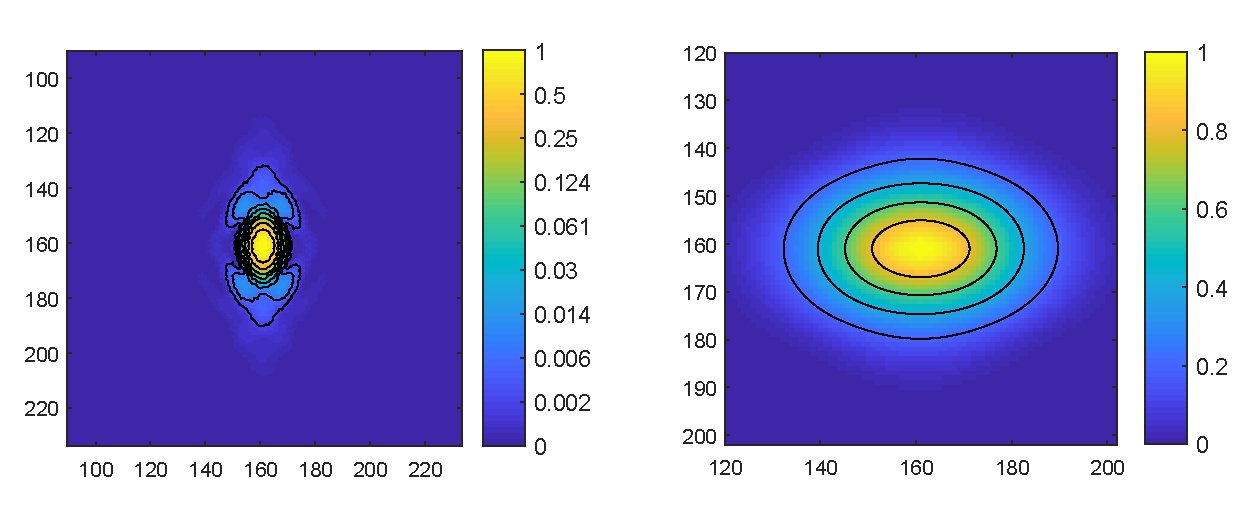
\includegraphics[width=1\textwidth]{psfs/SPIMx120.pdf}
    \bcaption[Axial cross section of the PSF and OTF of a multi-view single plane illumination microscope]{Simulated PSF and OTF for a single plane illumination microscope with a water immersion objectives ($n=1.33$). Muti-view image acquisition at \SI{120}{\degree} was simulated. Detection: $NA=1.1$, $\lambda = \SI{510}{nm}$, Illumination: $NA=0.1$, $\lambda = \SI{488}{nm}$}
    \label{fig:psf-spimx120}
\end{figure}
    


\section{Optical layout}
design principles:
highest isotropic resolution, highest light collection efficiency possible
2x0.8 NA water dipping in 90$\circ$ multi-view deconvolve Gaussian fit $\sigma_{xyz}=135$
2x1.1 NA water dipping in 120$\circ$ multi-view deconvolced Gaussian fit $\sigma_z = 135$, and $\sigma_{xy} = 82.2$
simulations from PSF generator! put here

\begin{figure}[bth]
    \centering
    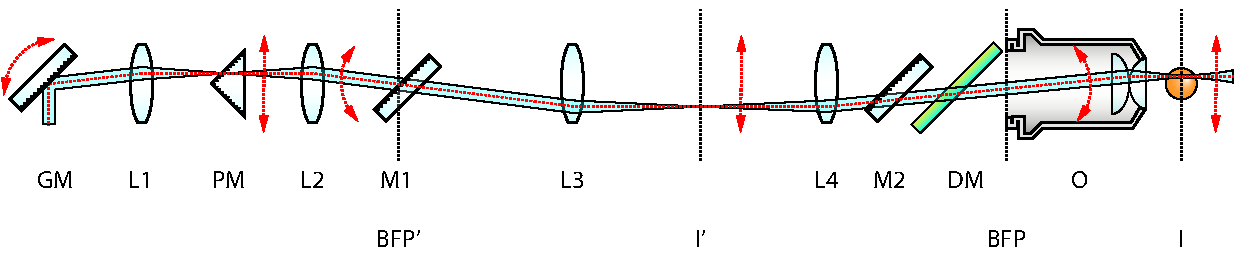
\includegraphics[page=1,width=1\textwidth]{schematicsLinear}
    \bcaption[Simplified schematics for illumination]{}
    \label{fig:schematicsLinear}
\end{figure}

When designing the optical layout of the setup, we had two principles in mind: simplicity and efficiency. Because of the symmetrical design it is possible that


\section{Optical alignment}
Precise alignment of the illumination and detection paths are crucial for high quality imaging, and has a pronounced  importance for high magnification and high resolution optical systems. The DualMouse SPIM contains two illumination and detection paths that share many common elements, which makes alignment a *important?* process. The final aim for the alignment is to perfectly overlap the light-sheets with the detection focal planes, and to optimize ... 

\subsection{Alignment of illuminaiton branches}

The two illumination braches start with a common light source, a single mode fiber coupled to laser combiner, and they also share a galvanometric mirror that performs the beam scanning to generate the virtual light-sheet. Likewise shared is a scan lens focusing on the galvo mirror (GM), and the illumination splitter unit (PM, see Section \ref{sec:splitter}).

Alignment for the illumination arms are done in three steps. First the laser beam is aligned on the first rail that holds the galvo, lens L1, and the splitter unit PM. This is performed by two kinematic mirrors placed between the fiber output and the galvo mirror. Using these two mirrors it's possible to freely align the beam along all 4 degrees of freedom: translation in two orthogonal directions, and rotation around two orthogonal axes. Beam alignment on the rail is tested by two irises at the two ends of the rail, if the beam passes through both of them we consider it centered and straight on the optical axis.

After the beam is aligned on the first rail, lens L1 and the splitter unit PM are placed in the measured positions to image the galvo mirror on mirror M1 using lenses L1 and L2. Correct positioning of the splitter unit along the rail is crucial, since this will affect the lateral position and tilt of the beam exiting the unit. To some extent, this can also be compensated by adjusting the two mirrors before the galvo mirror, but is avoided if possible as this will also displace the beam from the center of the galvo mirror.

\paragraph{Adjusting beam position.}
Beam position can be adjusted by either translating the beam in a conjugated image plane, or by rotating the beam in a conjugated back focal plane. The setup was designed in a way, that BFP' coincides with mirror M2. This mirror is mounted in a gimbal mirror mount, allowing to rotate the mirror exactly around its center, which avoids unwanted translational movements, and results in pure rotation of the beam. Lens L3 is positioned exactly 1 focal length from the mirror, thus acting as a scan lens, and transforming the rotational movements to translation. This translation is further imaged and demagnified by the tube lens L4 and the objective O.


\paragraph{Adjusting beam tilt}
Beam tilt can be adjusted by 



\paragraph{Adjusting beam axial position.}


\paragraph{Adjusting scanning plane angle.}
After the beam is properly aligned, i.e. it is in focus, and in the center of filed of view, it is still necessary to check if the scanning direction is parallel to the imaging plane. It is possible that the beam is in focus in the center position, but when moved up or down it drifts out of focus due to a tilted scanning angle. This tilt can be compensated by mirror M1, that is placed at the conjugated back focal plane BFP'. Between lenses L3 and L4 a magnified version of the light-sheet will be visible, and the tilt can be checked by placing an alignment target in the optical path while scanning the beam. By tilting mirror M1 up or down, the scanning pattern not only moves up or down, but is also rotated if the mirror surface is not exactly vertical. Since M1 and GM are in conjugated planes, the tilt and offset can be performed independently. The tilt is first fixed by M1 while inspecting the target, and the beam is re-centered by changing the offset on the galvo mirror. Moving the galvo mirror will not introduce tilt, since in this case rotation axis is perpendicular to the reflection plane.





\subsection{Alignment of detection branches}
Since the detection path is equivalent to a wide-field detection scheme, its alignment is much simpler than that of the illumination branches. The only difference is the detection branch merging unit (see Sec. \ref{sec:dualMirror}.) that features two moving mirrors. This, however doesn't effect the alignment procedure, since the movement direction is parallel to both mirror's surface, meaning that the exact position of the mirrors will not affect the image quality, as long as the mirrors are not clipping the image itself. Stability test were performed to confirm the consistent switching performance of the mirror unit before the final alignment took place (see Sec. \ref{sec:mirrorStability}).

% TODO: complete paragraph
The final alignment procedure 

\paragraph{Positioning the tube lens.}
The position of the tube lens determines the focal plane the is being imaged on the camera sensor. Ideally, the tube lens' distance from the camera sensor is exactly the tube lens focal length, which will ensure the best imaging performance. If the tube lens distance is not correct, the focal plane will be slightly shifted in the axial direction. Although small shifts will not necessarily have detrimental effect on the image quality, because the light sheet can also be shifted accordingly. Because of the shifted focal and image planes, however, the magnification of the system will be affected, and will change depending on the amount of defocus. For this reason we aim for positioning the tube lens as close to the theoretical position as possible.

Our tube lens is a compound, achromatic lens with a center thickness of \SI{12.5}{mm}, and edge thickness of \SI{11.3}{mm}. Its effective focal length is \SI{400}{mm} which will produce a 50x magnified image. Back focal length is \SI{394.33}{mm} which we measured form the camera chip, and the lens was positioned at this theoretically optimal position.

\paragraph{Adjusting correction collar.}
The Nikon 25x objectives used for this setup have a built in correcction ring that can be used to correct spherical aberrations resulting from refractive index differences when imaging samples behind a coverslip. This can be also effectively used to correct for any spherical aberrations occurring from imaging through the FEP foil. Although these aberrations are expected to be extremely low, due to the relatively thin, \SI{50}{\micro m} foil thickness, and the close matching of refractive index ($n_{FEP} = 1.344$, $n_{H_2O}=1.333$), for optimal, aberration free image quality it can't be neglected.

The correction collars are adjusted by inspecting a gel suspended fluorescent bead specimen with the microscope, where the beads can act as a reporter of the point spread function of the microscope. The alignment can be performed "live" by inspecting the bead image quality for any aberrations. By gradually changing the correction collar, the ring are minimized on out of focus beads, and the peak intensity is maximized for in focus beads. By moving the correction ring, the focal plane is also slightly shifted, which has to be compensated by shifting the light-sheet correspondingly to coincide with the correct imaging plane.

\paragraph{Adjusting field of view.}
To allow for proper sampling of the image, we use 50x magnification, which, combined with the \SI{6.5}{\micro m} pixel pitch of our sCMOS camera will result in a \SI{0.13}{\micro m} pixel size. The full field of view with this magnification is $2048 \times 0.13 = \SI{266.24}{\micro m}$. The full field of view the objective provide, are larger than this, at \SI{800}{\micro m}. To ensure the best image quality, we align the center of the objective field of view on the camera sensor, since this region has the best optical properties in term of numerical aperture, aberration correction and field flatness.

Field of view alignment can be performed using mirror M4 just before the detection merging unit. To identify the center region of the field of view, diffuse white light is used to illuminate the entire sample chamber, and is imaged on the camera. Then, mirror M4 is adjusted until the top edge of the field of view becomes visible, \textit{i.e.} where the illumination from the chamber is clipped. This will have a circular shape. Then, adjusting the mirror in the orthogonal direction, the left-right position of the field of view can be adjusted, by centering the visible arc on the camera sensor.

After the horizontal direction is centered, vertical centering is performed. This, however can't be centered the same way as the horizontal direction, since for that we would have to misalign the already aligned horizontal position. To determine the center, we move the field of view from the topmost position to the bottom. During this process the number of  turns of the adjustment screw is counted (this can be done accurately by using a hex key). After reaching the far end of the field of view, the mirror movement is reversed, and the screw is turned halfway to reach the middle.

\begin{figure}[hbt]
    \centering
    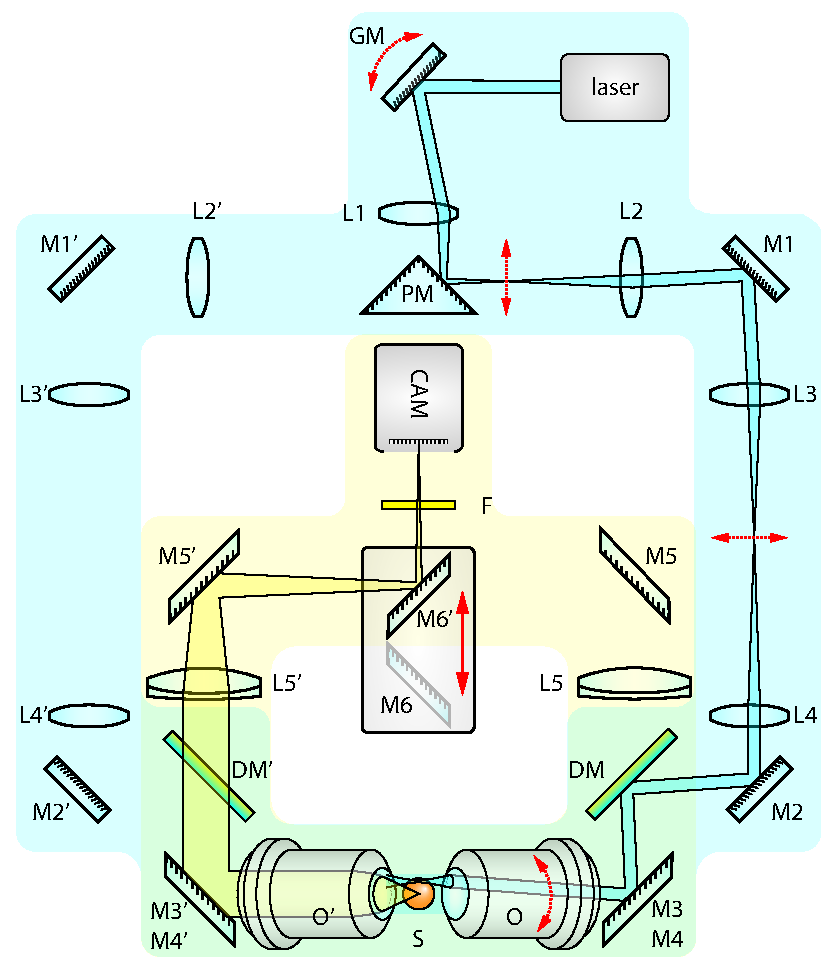
\includegraphics[page=1,width=1\textwidth]{fullSchematics}
    \bcaption[Dual Mouse SPIM optical layout]{The microscope consists of two main parts, the illumination branches (blue) and detection branches (yellow). For both illumination and detection there are two identical paths implemented. Illumination direction can be changed by applying a different offset to the galvo mirror, which in turn will direct the beam to the opposite face of the prism mirror. L1 and L2 will then image the galvo on M1. Using L3 as a scan lens, and L4 as a tube lens, the scanned beam is coupled to the objective path by quad band dichroic mirror (DM)
    CAM -- camera, DM -- dichroic mirror, F -- filter wheel, L -- lens, M -- mirror, O -- objective, PM -- prism mirror, S -- sample, SU -- switcher unit 
}
    \label{fig:fullSchematics}
\end{figure}

\subsection{3D figures}
\subsection{Illuminaiton splitter unit}
\label{sec:splitter}
\begin{figure}[htb]
    \centering
    \includemedia[
    width=0.8\linewidth,height=0.6\linewidth,
    %add3Djscript=asylabels.js, %upright text labels
    %add3Djscript=3Dspintool.js, %let scene rotate about z-axis
    % 3Dcoo, 3Droo values found with `Generate Default View' from
    % context menu
    3Dmenu,
    playbutton=plain,
    3Droll=124.45821807473328,
    3Dc2c=0.5729350447654724 0.4988637864589691 0.6502924561500549,
    3Dcoo=6.723448276519775 -30.282148361206055 -11.914359092712402,
    3Droo=162.71372963736036,
    3Dlights=Headlamp,
    3Drender=ShadedIllustration,
    ]{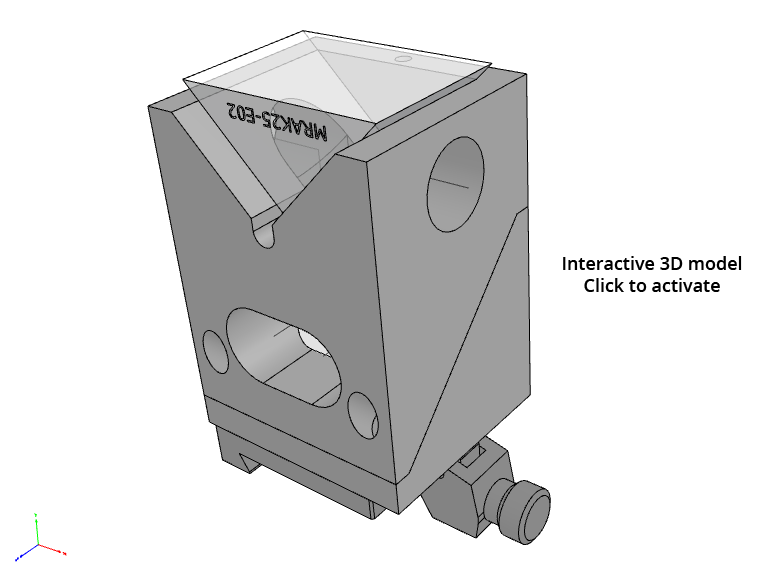
\includegraphics{Splitter.png}}{Splitter.prc}
\bcaption[Illumination branch splitting block]{3D model of the custom designed splitter block used in the illumination branch. Depending on the horizontal beam position at the lower port, the beam will be reflected either to the right or to the left. Because of the mirror alignment, the beam is rotated 90 degrees.}
\label{fig:splitter}
\end{figure}

\subsection{Detection merging unit}
\label{sec:dualMirror}

\begin{figure}[htb]
\centering
    \includemedia[
width=1.0\linewidth,height=0.6\linewidth,
%add3Djscript=asylabels.js, %upright text labels
%add3Djscript=3Dspintool.js, %let scene rotate about z-axis
% 3Dcoo, 3Droo values found with `Generate Default View' from
% context menu
3Dmenu,
playbutton=plain,
% default view start
3Droll=104,
3Dc2c=0.7466059923171997 0.4799830913543701 0.4606471359729767,
3Dcoo=-5.2039947509765625 -5.257904529571533 23.018417358398438,
3Droo=353,
3Dlights=Headlamp,
3Drender=ShadedIllustration,
% default view end
]{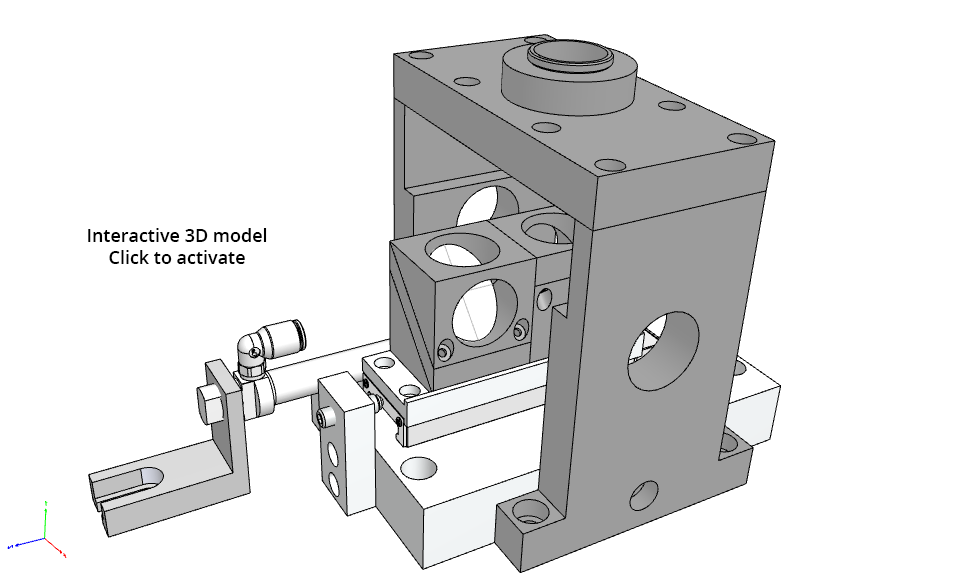
\includegraphics{DualMirror.png}}{DualMirror.prc}
\caption[Detection branch merging unit]{3D model of the custom designed unit to enable quick switching between the two detection paths. A high precision stainless steel stage holds two mirror blocks facing opposite directions, and bouncing the light upwards, towards the camera. The units are translated by  pneumatic cylinder to ensure high speed an reproducibility.}
\label{fig:DualMirror}
\end{figure}

\section{Results}
\begin{figure}[htb]
    \begin{subfigure}[t]{0.5\textwidth}
        \centering
        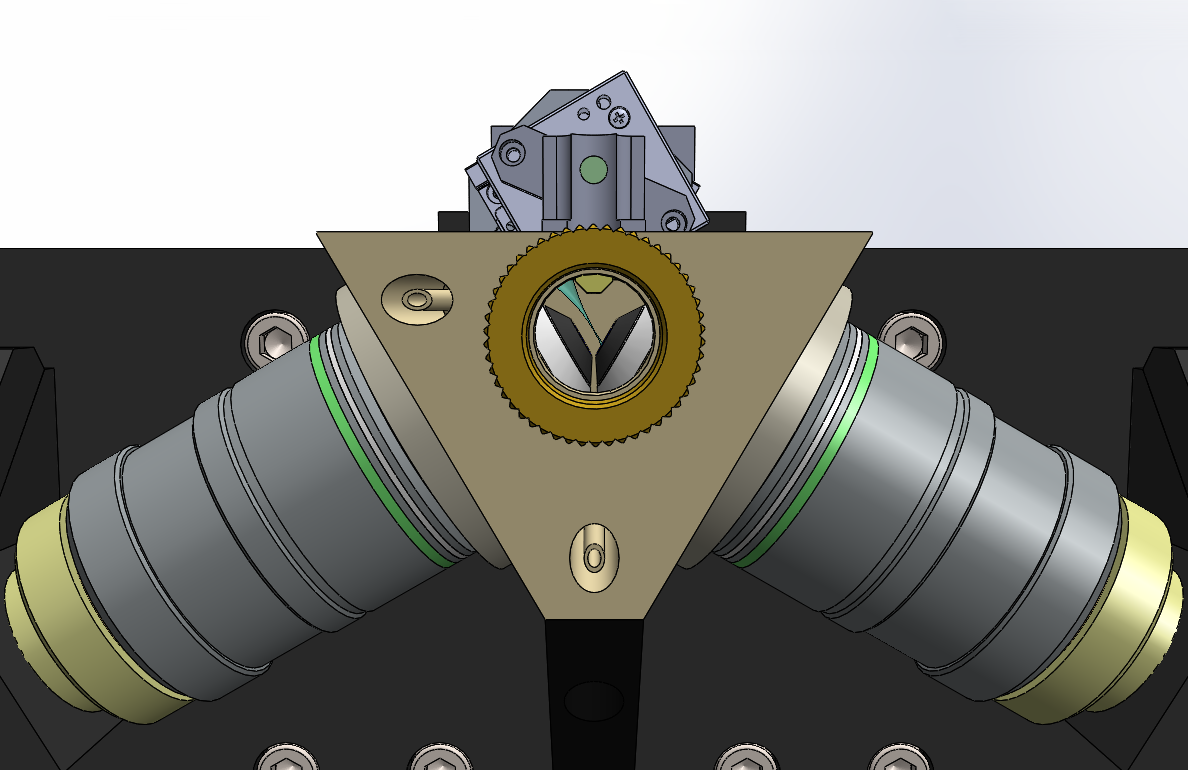
\includegraphics[width=\textwidth]{front_solidworks_overlay}
        \caption{Rendering of SolidWorks design.}
    \end{subfigure}
    \begin{subfigure}[t]{0.5\textwidth}
        \centering
        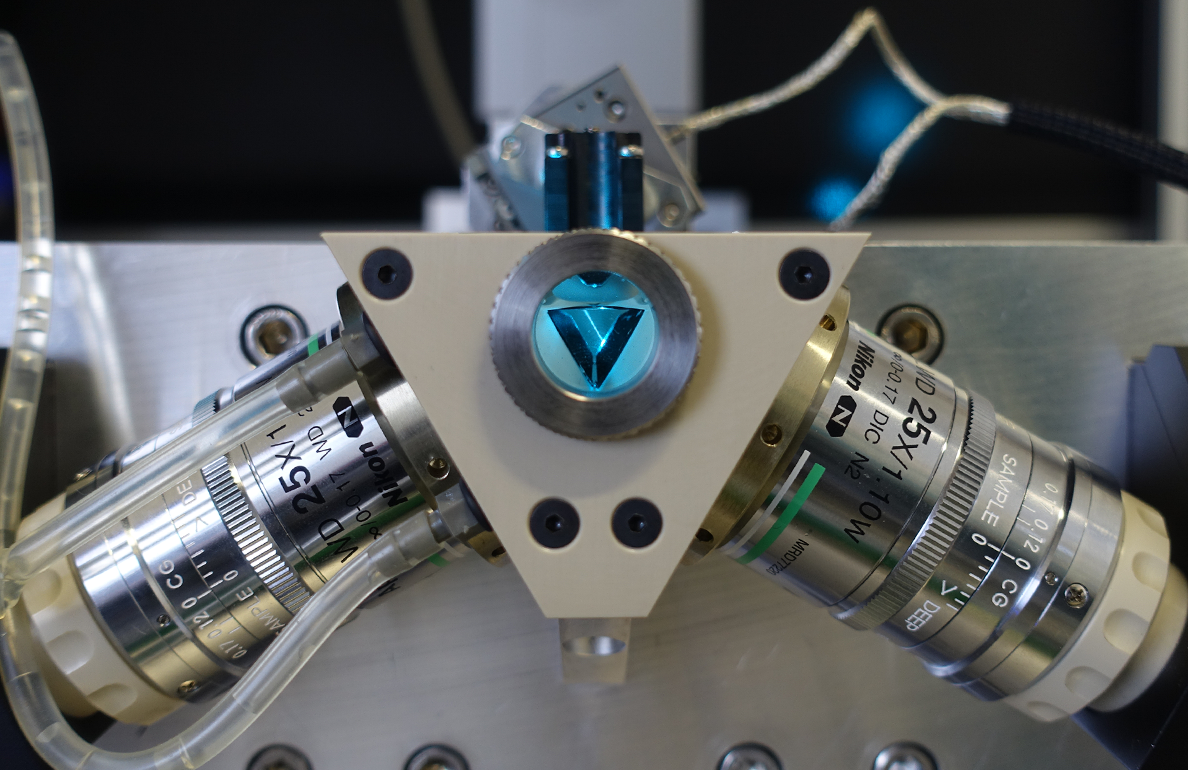
\includegraphics[width=\textwidth]{front_photo_overlay}
        \caption{Photo of constructed microscope.}
    \end{subfigure}
    \bcaption[Front view of the Dual Mouse-SPIM]{}
    \label{fig:frontView}
\end{figure}

Resolution for Lattice light-sheet \cite{chen_lattice_2014}: \SI{230}{nm} in x and \SI{370}{nm} in z
\cite{chhetri_whole-animal_2015}

\begin{figure}[htb]
    \centering
    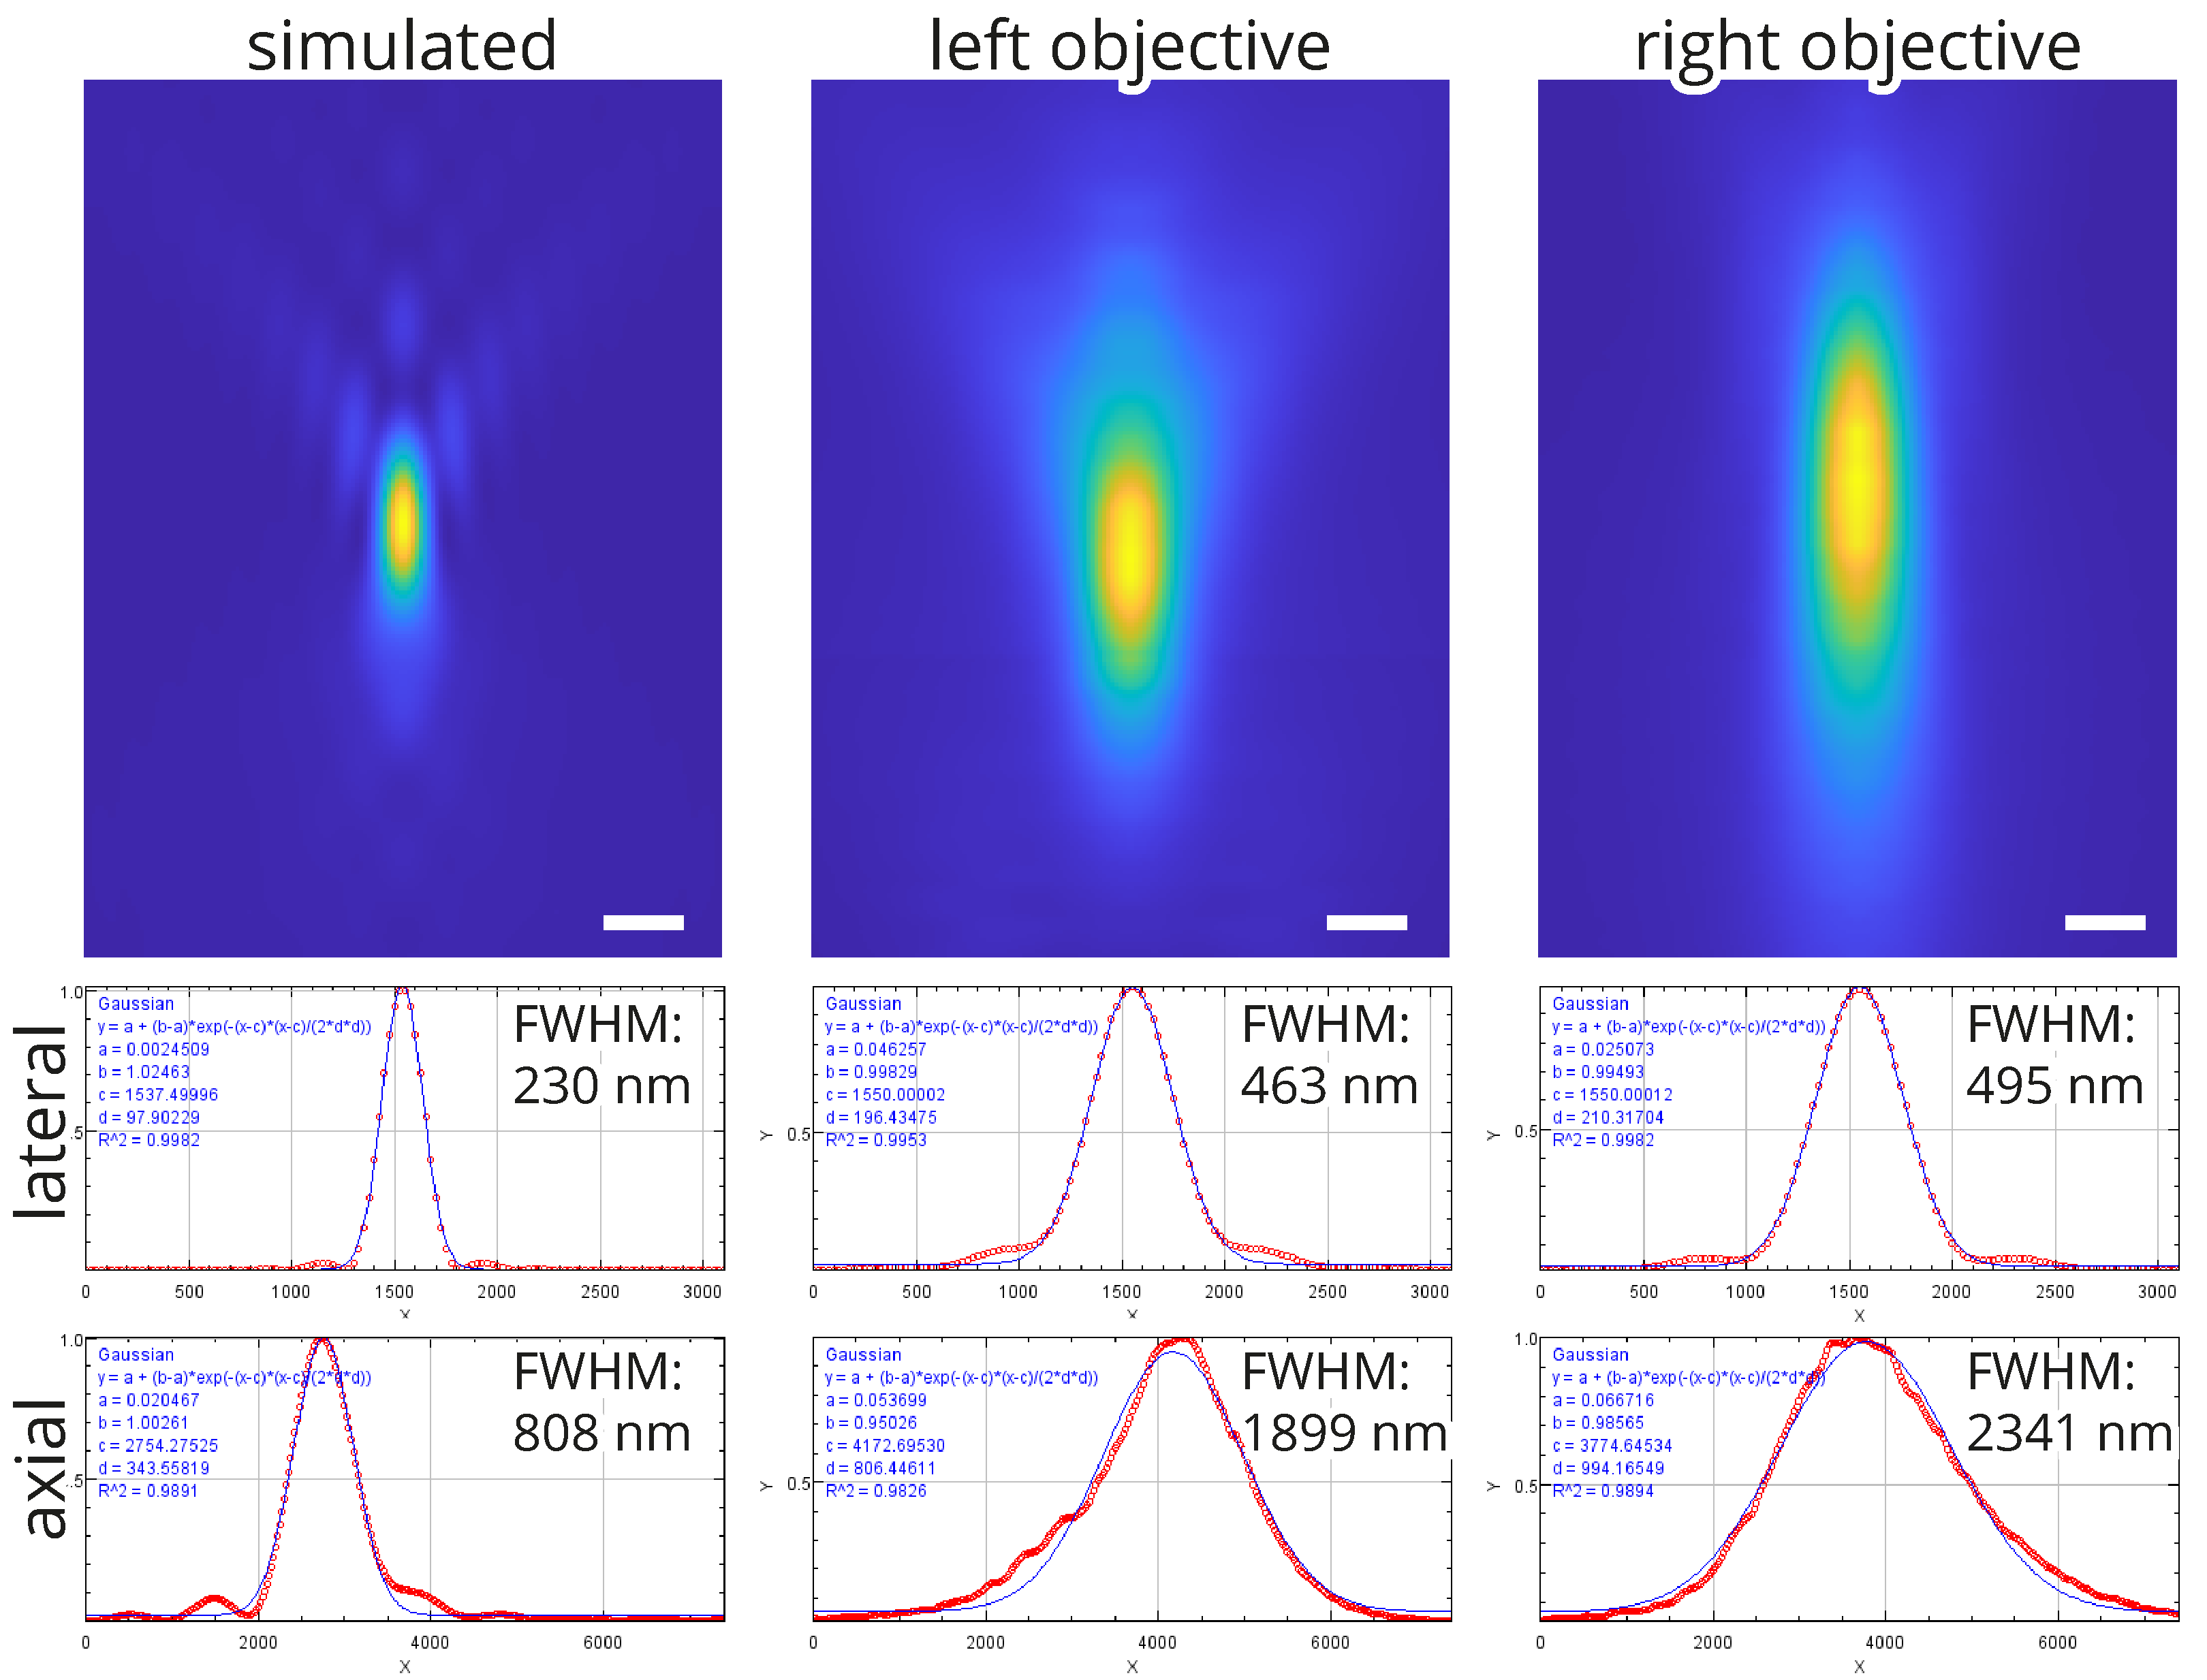
\includegraphics[width=\textwidth]{PSF}
    \bcaption[Simulated and measured PSF of Dual Mouse-SPIM]{Top row: axial sections of simulated and measured point spread funcitons. Middle row: lateral intensity profile and Gaussian fit. Bottom row: Axial intensity profile and Gaussian fit. Simulations were performed based on the Gibson-Lanni model. Immersion medium  and sample refractive index: 1.330, coverslip (FEP foil) refractive index: 1.344, coverslip distance: \SI{1900}{\micro m}, coverslip thickness: \SI{50}{\micro m}. Scale bar: \SI{500}{nm}.}
\end{figure}